\documentclass[12pt, oneside, openany]{article}
\usepackage[T1]{fontenc}
\usepackage[spanish, es-tabla, es-lcroman]{babel}
\usepackage[utf8]{inputenc}
\usepackage[document]{ragged2e}
\usepackage{tcolorbox}
\tcbuselibrary{theorems}
\usepackage{cancel}
\usepackage{amssymb}
\usepackage{amsmath}
\usepackage{mathrsfs}
\usepackage{wrapfig}
\usepackage{fancyhdr}
\usepackage{colortbl}
\usepackage{longtable}
\usepackage{diagbox}
\usepackage{graphicx}
\usepackage{subcaption}
\usepackage{xcolor}
\usepackage{tikz}
\usetikzlibrary{positioning}
\usepackage{multicol}
\usepackage{multirow}
\usepackage{lastpage}
\usepackage{pdfpages}
\usepackage{listings}
\usepackage{blindtext}
\spanishdecimal{.}
\usepackage[explicit]{titlesec}
\usepackage[colorlinks=true, linkcolor=black, citecolor=black, urlcolor=blue]{hyperref}
\usepackage[a4paper, total={16cm, 24cm}]{geometry}
\pagestyle{fancy}
\lhead{Muñoz Nulez Ian Emmanuel}
\rhead{Proyecto 7}
\lfoot{Mtra. María Patricia Ventura Nuñez}
\rfoot{CUCEI}
\renewcommand{\headrulewidth}{1pt}
\renewcommand{\footrulewidth}{1pt}

\setlength{\headheight}{14.49998pt}

\begin{document}

\begin{titlepage}
    \pagenumbering{roman}
    \centering
    {\bfseries\LARGE Universidad de Guadalajara \par}
    \vfill
    {
        \includegraphics[width=0.3\linewidth]{UdG.png}
        \includegraphics[width=0.3\linewidth]{qci.png}
        \par
    }
    \vfill
    {\bfseries\LARGE Seminario de problemas de programación de sistemas reconfigurables \par}
    \vfill
    {\LARGE Diseño e implementación de una maquina de estados utilizando Flip-Flop's y entradas asíncronas \par}
    \vfill
    {\bfseries\LARGE Nombre: \par}
    \vfill
    {\bfseries\LARGE Muñoz Nuñez Ian Emmanuel \par}
    \vfill
    {\bfseries\LARGE Sección: D01 \par}
    \vfill
    {\bfseries\LARGE Código: 216464457 \par}
    \vfill
    {\bfseries\LARGE Maestra: \par}
    \vfill
    {\bfseries\LARGE María Patricia Ventura Nuñez \par}
    \vfill
    {\bfseries\LARGE Ingeniería Robótica \par}
\end{titlepage}

\pagenumbering{arabic}

\newpage
\section{Objetivo}
{\sffamily\large
    \hspace{0.5cm} Solucionar problemas de diseño utilizando las herramientas aprendidas en programación de sistemas reconfigurables.
    
    \hspace{0.5cm} Simular circuitos digitales en programas de diseño como \emph{Proteus\textregistered} e implementarlos físicamente.
    
    \hspace{0.5cm} Diseño e implementación de una maquina de estados utilizando Flip-Flop's y entradas asíncronas.
    
}

\section{Material}
{\sffamily\large
    \renewcommand{\labelitemi}{$\bullet$}
    \begin{itemize}
        \item Protoboard.
        \item Fuente VCC (5V).
        \item Resistencias de $200\Omega$ y $2k\Omega$.
        \item Dip switch de 8 bits.
        \item 3 leds.
        \item 2 Flip-Flop's 4027.
        \item 1 GAL22v10.
    \end{itemize}
}

\newpage
\section{Marco teórico}
\subsection{Tablas de verdad para Flip-Flop's}
{\sffamily\large
    \begin{table}[h!]
        \centering
        \sffamily
        \scalebox{1.3}{
        \begin{tabular}{|c|c|c|c||c|}
            \hline
            \multicolumn{5}{|c|}{SR} \\
            \hline
            & S & R & $Q^t$ & $Q^{t+1}$ \\
            \hline
            \multirow{8}{*}{Nivel alto} & 0 & 0 & 0 & 0 \\
            \cline{2-5}
            & 0 & 0 & 1 & 1 \\
            \cline{2-5}
            & 0 & 1 & 0 & 0 \\
            \cline{2-5}
            & 0 & 1 & 1 & 0 \\
            \cline{2-5}
            & 1 & 0 & 0 & 1 \\
            \cline{2-5}
            & 1 & 0 & 1 & 1 \\
            \cline{2-5}
            & 1 & 1 & 0 & X \\
            \cline{2-5}
            & 1 & 1 & 1 & X \\
            \hline
            \multirow{8}{*}{Nivel bajo} & 0 & 0 & 0 & X \\
            \cline{2-5}
            & 0 & 0 & 1 & X \\
            \cline{2-5}
            & 0 & 1 & 0 & 1 \\
            \cline{2-5}
            & 0 & 1 & 1 & 1 \\
            \cline{2-5}
            & 1 & 0 & 0 & 0 \\
            \cline{2-5}
            & 1 & 0 & 1 & 0 \\
            \cline{2-5}
            & 1 & 1 & 0 & 0 \\
            \cline{2-5}
            & 1 & 1 & 1 & 1 \\
            \hline
        \end{tabular}
        }
        \caption{\sffamily Tabla de verdad \emph{SR}}
        \label{tab:tablaSR}
    \end{table}
    
    \begin{table}[h!]
        \centering
        \sffamily
        \scalebox{1.3}{
        \begin{tabular}{|c|c||c|}
            \hline
            \multicolumn{3}{|c|}{D}\\
            \hline
            D & $Q^t$ & $Q^{t+1}$ \\
            \hline
            0 & 0 & 0 \\
            \hline
            0 & 1 & 0 \\
            \hline
            1 & 0 & 1 \\
            \hline
            1 & 1 & 1 \\
            \hline
        \end{tabular}
        }
        \caption{\sffamily Tabla de verdad \emph{D}}
        \label{tab:tablaD}
    \end{table}
    
}

\newpage
{\sffamily\large
    \begin{table}[h!]
        \centering
        \sffamily
        \scalebox{1.3}{
        \begin{tabular}{|c|c||c|}
            \hline
            \multicolumn{3}{|c|}{T} \\
            \hline
            T & $Q^t$ & $Q^{t+1}$ \\
            \hline
            0 & 0 & 0 \\
            \hline
            0 & 1 & 1 \\
            \hline
            1 & 0 & 1 \\
            \hline
            1 & 1 & 0 \\
            \hline
        \end{tabular}
        }
        \caption{\sffamily Tabla de verdad \emph{T}}
        \label{tab:tablaT}
    \end{table}
    
    \begin{table}[h!]
        \centering
        \sffamily
        \scalebox{1.3}{
        \begin{tabular}{|c|c|c|c||c|}
            \hline
            CK & J & K & $Q^t$ & $Q^{t+1}$ \\
            \hline
            0 & 0 & 0 & 0 & 0 \\
            \hline
            0 & 0 & 0 & 1 & 1 \\
            \hline
            0 & 0 & 1 & 0 & 0 \\
            \hline
            0 & 0 & 1 & 1 & 1 \\
            \hline
            0 & 1 & 0 & 0 & 0 \\
            \hline
            0 & 1 & 0 & 1 & 1 \\
            \hline
            0 & 1 & 1 & 0 & 0 \\
            \hline
            0 & 1 & 1 & 1 & 1 \\
            \hline
            1 & 0 & 0 & 0 & 0 \\
            \hline
            1 & 0 & 0 & 1 & 1 \\
            \hline
            1 & 0 & 1 & 0 & 0 \\
            \hline
            1 & 0 & 1 & 1 & 0 \\
            \hline
            1 & 1 & 0 & 0 & 1 \\
            \hline
            1 & 1 & 0 & 1 & 1 \\
            \hline
            1 & 1 & 1 & 0 & 1 \\
            \hline
            1 & 1 & 1 & 1 & 0 \\
            \hline
        \end{tabular}
        }
        \caption{\sffamily Tabla de verdad \emph{JK}}
        \label{tab:tablaJK}
    \end{table}
    
}

\newpage
\subsection{Tabla de activación}
{\sffamily\large
    \begin{table}[h!]
        \centering
        \sffamily
        \scalebox{1.3}{
        \begin{tabular}{|c|c||c|c|c|c|c|c|}
            \hline
            $Q^t$ & $Q^{t+1}$ & S & R & J & K & T & D \\
            \hline
            0 & 0 & 0 & X & 0 & X & 0 & 0 \\
            \hline
            0 & 1 & 1 & 0 & 1 & X & 1 & 1 \\
            \hline
            1 & 0 & 0 & 1 & X & 1 & 1 & 0 \\
            \hline
            1 & 1 & X & 0 & X & 0 & 0 & 1 \\
            \hline
        \end{tabular}
        }
        \caption{\sffamily Tabla de activación}
        \label{tab:tablaActivacion}
    \end{table}
    
}

\subsection{Tabla de verdad del circuito}
{\sffamily\large
    \begin{table}[h!]
        \centering
        \sffamily
        \begin{tabular}{|c||c|c|c||c|c|c||c|c||c|c||c|c||c|c|}
            \hline
            & \multicolumn{3}{c||}{$Q^t$} & \multicolumn{3}{c||}{$Q^{t+1}$} & \multicolumn{2}{c||}{A} & \multicolumn{2}{c||}{B} & \multicolumn{2}{c||}{C} \\
            \hline
            X & QA & QB & QC & QA & QB & QC & JA & KA & JB & KB & JC & KC \\
            \hline\hline
            0 & 0 & 0 & 0 & X & X & X & X & X & X & X & X & X \\
            \hline
            0 & 0 & 0 & 1 & 1 & 1 & 1 & 1 & X & 1 & X & X & 0 \\
            \hline
            0 & 0 & 1 & 0 & X & X & X & X & X & X & X & X & X \\
            \hline
            0 & 0 & 1 & 1 & 1 & 0 & 0 & 1 & X & X & 1 & X & 1 \\
            \hline
            0 & 1 & 0 & 0 & 1 & 1 & 0 & X & 0 & 1 & X & 0 & X \\
            \hline
            0 & 1 & 0 & 1 & X & X & X & X & X & X & X & X & X \\
            \hline
            0 & 1 & 1 & 0 & 0 & 0 & 1 & X & 1 & X & 1 & 1 & X \\
            \hline
            0 & 1 & 1 & 1 & 0 & 1 & 1 & X & 1 & X & 0 & X & 0 \\
            \hline\hline
            1 & 0 & 0 & 0 & X & X & X & X & X & X & X & X & X \\
            \hline
            1 & 0 & 0 & 1 & 1 & 1 & 0 & 1 & X & 1 & X & X & 1 \\
            \hline
            1 & 0 & 1 & 0 & X & X & X & X & X & X & X & X & X \\
            \hline
            1 & 0 & 1 & 1 & 1 & 1 & 1 & 1 & X & X & 0 & X & 0 \\
            \hline
            1 & 1 & 0 & 0 & 0 & 1 & 1 & X & 1 & 1 & X & 1 & X \\
            \hline
            1 & 1 & 0 & 1 & X & X & X & X & X & X & X & X & X \\
            \hline
            1 & 1 & 1 & 0 & 1 & 0 & 0 & X & 0 & X & 1 & 0 & X \\
            \hline
            1 & 1 & 1 & 1 & 0 & 0 & 1 & X & 1 & X & 1 & X & 0 \\
            \hline
        \end{tabular}
        \caption{\sffamily Tabla de verdad del circuito}
        \label{tab:tablaCircuito}
    \end{table}
    
}

\newpage
\section{Procedimiento}
{\sffamily\large
    \hspace{0.5cm} Primero se obtuvo la tabla de verdad y después las ecuaciones lógicas para armar el circuito.
    
    \hspace{0.5cm} Armar este circuito fue un poco confuso, pues se tienen entradas retro-alimentadas, por lo que es difícil entender como hacer las conexiones al principio.
    
    \hspace{0.5cm} Los materiales utilizados son: 1 dip switch de 8 bits, 2 resistencias de $2k\Omega$ y 3 de $220\Omega$, 3 leds, 2 \emph{Flip-Flop's 4027}, una \emph{GAL22v10D} y un generador de una señal de reloj.
    
}

\section{Circuito a implementar}
\subsection{Simulación}
{\sffamily\large
    \hspace{0.5cm} En la siguiente página se muestra el diseño del circuito en simulación.
    
    \newpage
    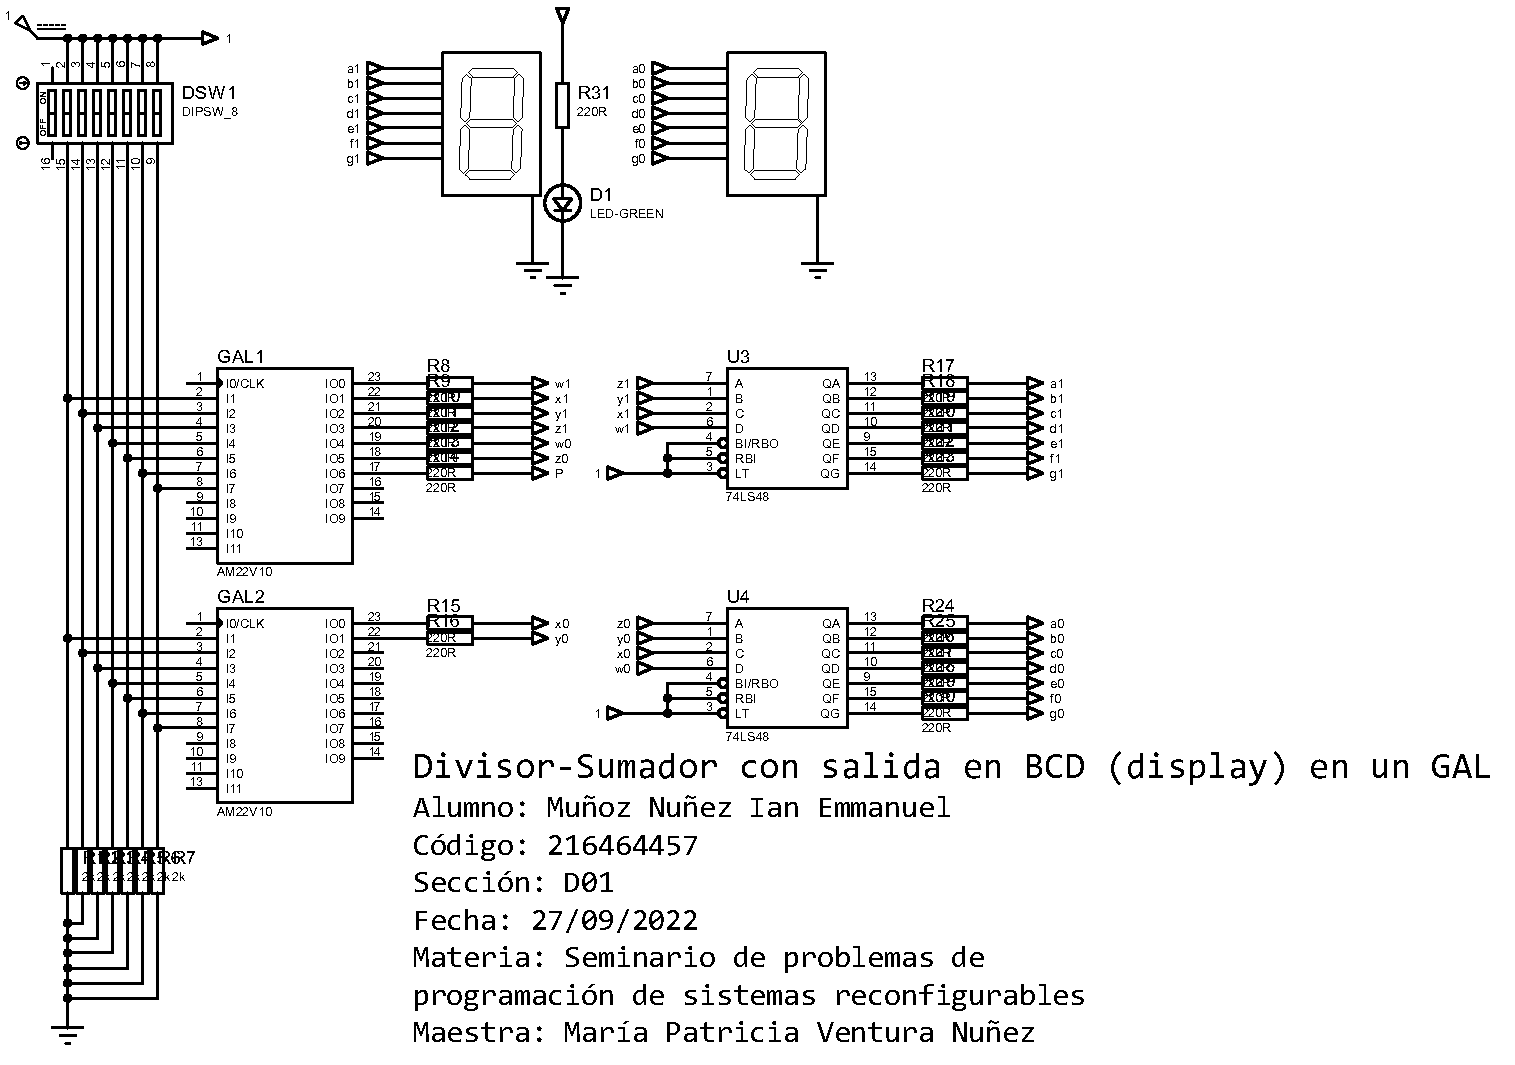
\includepdf[pages={1}]{main.PDF}
}

\newpage
\subsection{Protoboard}
\begin{figure}[h!]
    \centering
    
    \begin{subfigure}[tl]{0.45\textwidth}
        \centering
        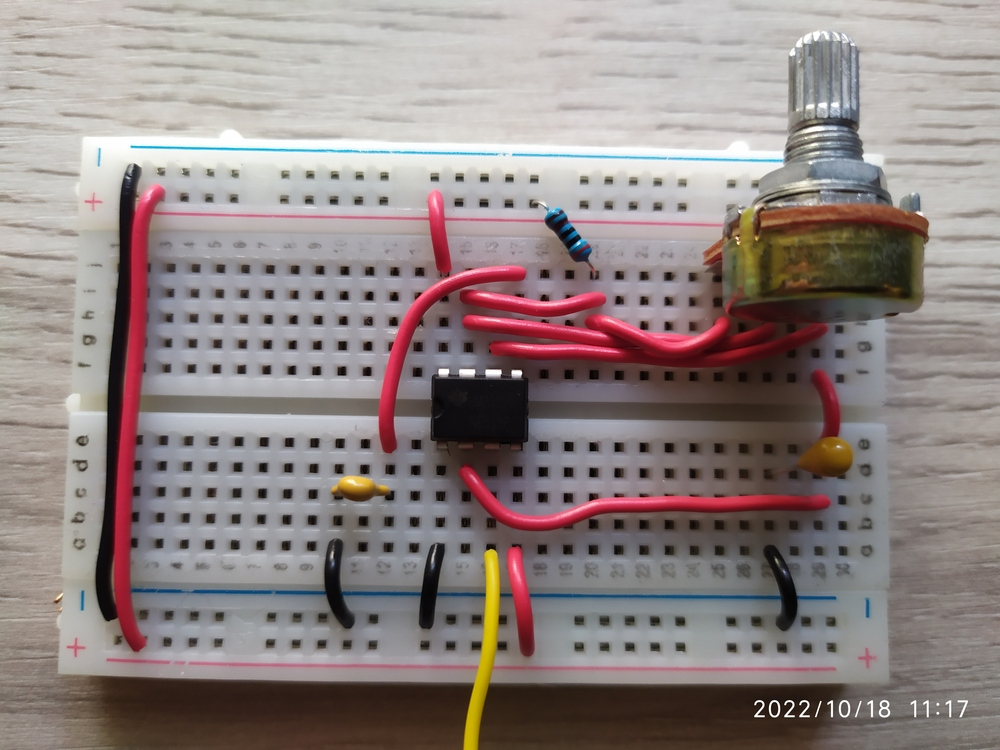
\includegraphics[width=\linewidth]{IMG_20221018_111718.jpg}
    \end{subfigure}
    \begin{subfigure}[tr]{0.45\textwidth}
        \centering
        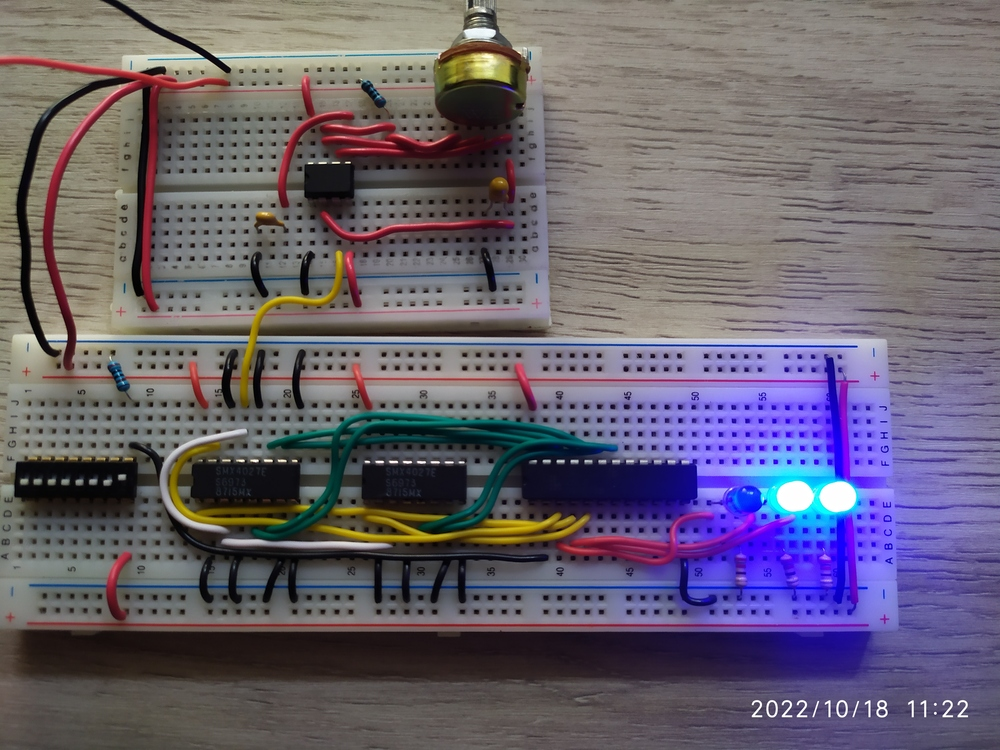
\includegraphics[width=\linewidth]{IMG_20221018_112237.jpg}
    \end{subfigure}
    \begin{subfigure}[bl]{0.45\textwidth}
        \centering
        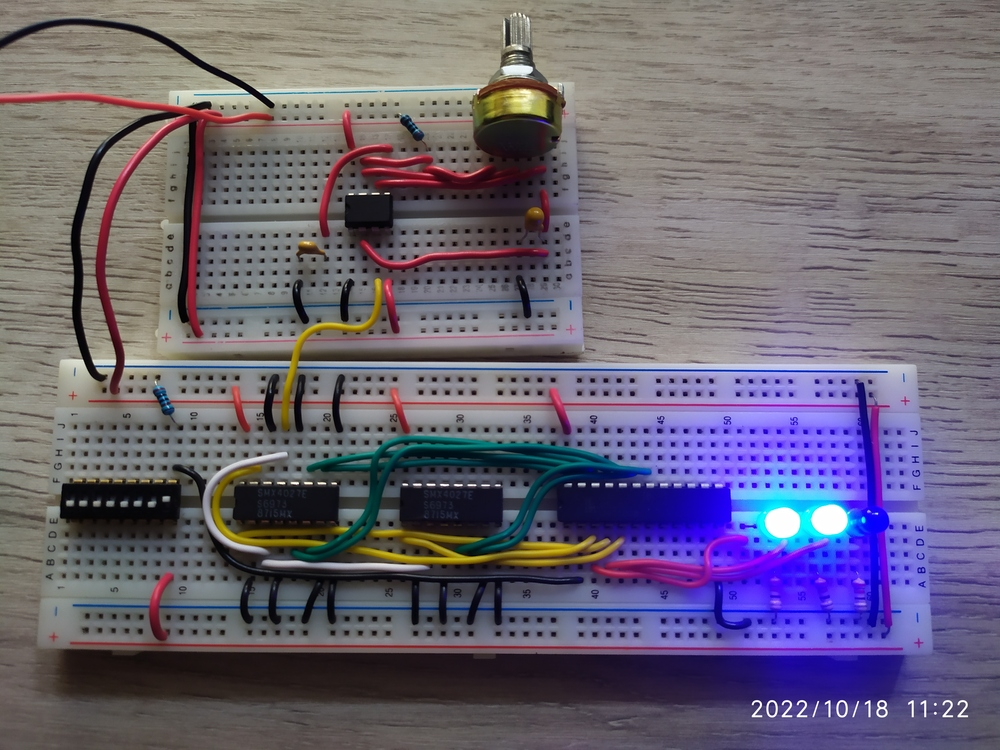
\includegraphics[width=\linewidth]{IMG_20221018_112242.jpg}
    \end{subfigure}
    \begin{subfigure}[br]{0.45\linewidth}
        \centering
        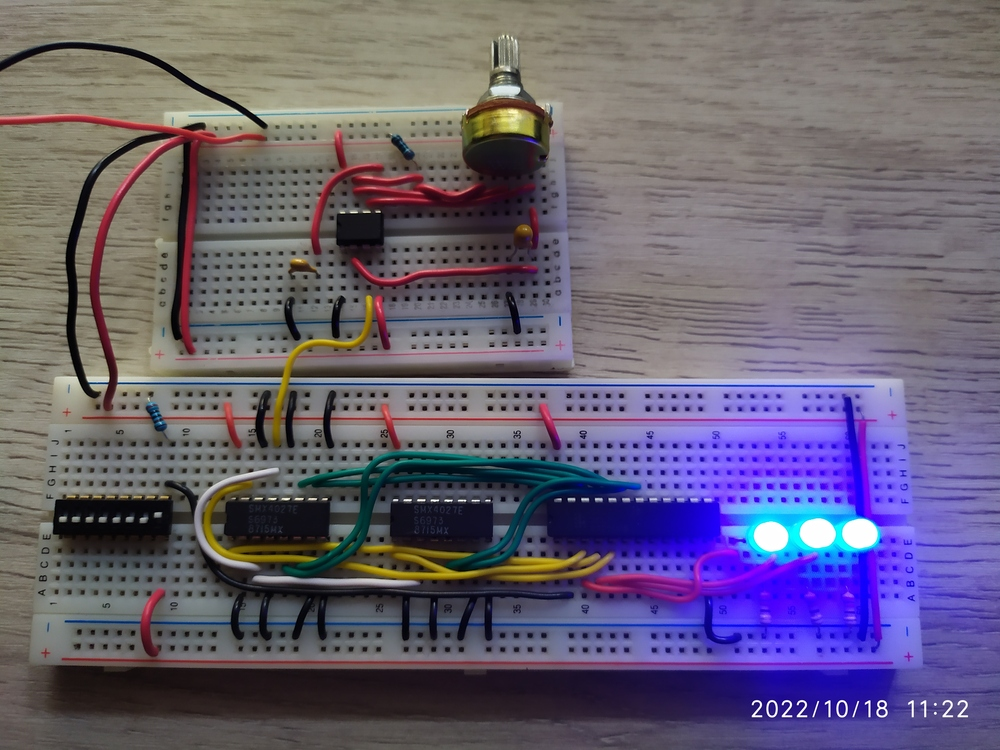
\includegraphics[width=\linewidth]{IMG_20221018_112250.jpg}
    \end{subfigure}
    
    \caption{\sffamily Circuito en protoboard}
    \label{fig:proto}
\end{figure}

\section{Conclusión}
{\sffamily\large
    \hspace{0.5cm} Comprender como funciona la lógica de este circuito fue complicado, pues entender el funcionamiento de las \emph{Flip-Flop's} cuesta un poco, pero una vez teniendo la tabla de verdad es sencillo seguir con el diseño del circuito.
    
}

\end{document}
